\documentclass[11pt,oneside]{article}
\usepackage[T1]{fontenc}
\usepackage[utf8]{inputenc}
%\DeclareUnicodeCharacter{00A0}{ }
\usepackage[adobe-utopia]{mathdesign}

\usepackage{amsmath}
\usepackage[francais]{babel}
\usepackage[dvips]{graphicx}
%\usepackage{here}
\usepackage{framed}
\usepackage[normalem]{ulem}
\usepackage{fancyhdr}
\usepackage{titlesec}
\usepackage{vmargin}

\usepackage{amsmath}
\usepackage{ifthen}
\usepackage{multirow}
\usepackage{multicol} % Portions de texte en colonnes

%\usepackage{xltxtra} % Logo XeLaTeX
%\usepackage{pst-solides3d}
\usepackage{color}
%\usepackage{colortbl}
\usepackage{titletoc} % Pour la mise en forme de la table des matières

%\usepackage[crop=off]{auto-pst-pdf}
%\usepackage{bclogo}


%\usepackage{longtable}
%\usepackage{flafter}%floatants après la référence
%\usepackage{pst-solides3d}
%\usepackage{pstricks}
%\usepackage{minitoc}
%\setcounter{minitocdepth}{4}
%\usepackage{draftcopy}% "Brouillon"
%\usepackage{floatflt}
%\usepackage{psfrag}
%\usepackage{listings} % Permet d'insérer du code de programmation
%\usepackage{lmodern}
%\usepackage[adobe-utopia,uppercase=upright,greeklowercase=upright]{mathdesign}
%\usepackage{minionpro}
%\usepackage{pifont}
%\usepackage{amssymb}
%\usepackage[francais]{varioref}

\setmarginsrb{1.5cm}{1cm}{1cm}{1.5cm}{1cm}{1cm}{1cm}{1cm}

\definecolor{gris25}{gray}{0.75}
\definecolor{bleu}{RGB}{18,33,98}
\definecolor{bleuf}{RGB}{42,94,171}
\definecolor{bleuc}{RGB}{231,239,247}
\definecolor{rougef}{RGB}{185,18,27}
\definecolor{rougec}{RGB}{255,230,231}
\definecolor{vertf}{RGB}{103,126,82}
\definecolor{vertc}{RGB}{220,255,191}
\definecolor{violetf}{RGB}{112,48,160}
\definecolor{violetc}{RGB}{230,224,236}
\definecolor{jaunec}{RGB}{220,255,191}

\usepackage[%
    pdftitle={SLCI -- Modélisation par schémas blocs -- Applications},
    pdfauthor={Xavier Pessoles},
    colorlinks=true,
    linkcolor=blue,
    citecolor=magenta]{hyperref}



% \makeatletter \let\ps@plain\ps@empty \makeatother
%% DEBUT DU DOCUMENT
%% =================
\sloppy
\hyphenpenalty 10000

\newcommand{\Pointilles}[1][3]{%
\multido{}{#1}{\makebox[\linewidth]{\dotfill}\\[\parskip]
}}


\begin{document}


\newboolean{prof}
\setboolean{prof}{false}
%------------- En tetes et Pieds de Pages ------------
\pagestyle{fancy}
\renewcommand{\headrulewidth}{0pt}

\fancyhead{}
\fancyhead[L]{%
\noindent\noindent\begin{minipage}[c]{2.6cm}
%Lycée Rouvière PTSI

\includegraphics[width=2cm]{png/logo_ptsi.png}%
\end{minipage}
}

\fancyhead[C]{\rule{12cm}{.5pt}}

\fancyhead[R]{%
\begin{minipage}[c]{3cm}
\begin{flushright}
\footnotesize{\textit{\textsf{Sciences Industrielles\\ de l'Ingénieur}}}%
\end{flushright}
\end{minipage}
}

\renewcommand{\footrulewidth}{0.2pt}

\fancyfoot[C]{\footnotesize{\bfseries \thepage}}
\fancyfoot[L]{\footnotesize{2013 -- 2014} \\ J.-P. \textsc{Pupier}}
\ifthenelse{\boolean{prof}}{%
\fancyfoot[R]{\footnotesize{CI 2 : SLCI -- Applications} \\ \footnotesize{Ch. 3 : Modélisation -- P}}
}{%
\fancyfoot[R]{\footnotesize{CI 2 : SLCI -- Applications} \\ \footnotesize{Ch. 3 : Modélisation -- E}}
}


%\begin{center}
%\textit{Centre d'intérêt}
%\end{center}



\begin{center}
 \Large\textsc{CI 2 -- SLCI : Étude du comportement des Systèmes Linéaires Continus Invariants}
\end{center}

\begin{center}
 \large\textsc{Chapitre 3 -- Modélisation des Systèmes Linéaires Continus Invariants}

 \large\textsc{Modélisation par schémas blocs} 
\end{center}

\begin{center}
\textsc{Exercices d'application} 

\end{center}

\begin{flushright}
\textit{D'après ressources de Jean-Pierre Pupier.} 
\end{flushright}
\vspace{.5cm}

\subsection*{Exercice 1}
On considère les systèmes représentés ci-dessous : 

\begin{minipage}[c]{.35\linewidth}
\begin{center}
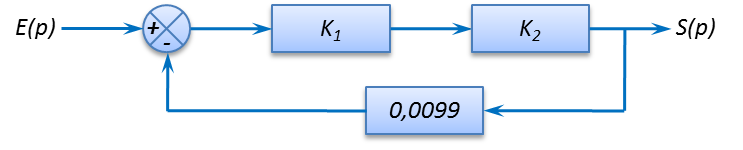
\includegraphics[width=\textwidth]{png/fig_01}
\end{center}
\end{minipage}\hfill
\begin{minipage}[c]{.6\linewidth}
\begin{center}
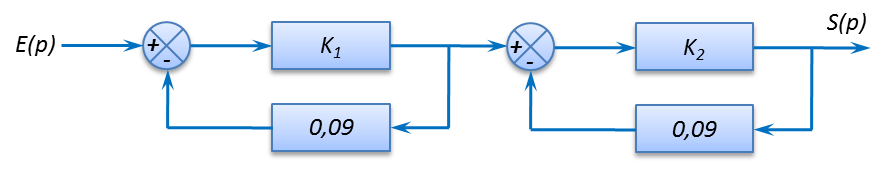
\includegraphics[width=.9\textwidth]{png/fig_02}
\end{center}
\end{minipage}

\vspace{.5cm}

Le premier système a pour fonction de transfert $H_1(p)$ et le deuxième $H_2(p)$. 

\subparagraph{}
\textit{Calculer $H_1(p)$ et $H_2(p)$.}

\ifthenelse{\boolean{prof}}{
\begin{corrige}
Dans le premier cas, on peut calculer la fonction de transfert en boucle fermée :
$$
H_1(p)=\dfrac{S(p)}{E(p)}=\dfrac{K_1(p)K_2(p)}{1+K_1(p)K_2(p) K_3}
$$

Dans le second cas, deux FTBF se succèdent. On a :
$$
H_2(p)=\dfrac{S(p)}{E(p)}=\dfrac{K_1(p)}{1+K_1(p) K_4}\cdot \dfrac{K_2(p)}{1+K_2(p) K_3}
= \dfrac{K_1(p) K_2(p)}{\left(1+K_1(p)K_4\right)\cdot\left(1+K_2(p)K_4\right)}
$$
\end{corrige}
}{}

\subparagraph{}
\textit{On pose $K_1=K_2=K$. Calculer $K$ tel que $H_1(p)=H_2(p)$.}

\ifthenelse{\boolean{prof}}{
\begin{corrige}
Dans le premier cas :
$$
H_1(p) = \dfrac{K^2}{1+K^2 K_3}
$$

Dans le second cas :
$$
H_2(p)= \dfrac{K^2}{\left(1+KK_4\right)\cdot\left(1+KK_4\right)}
= \dfrac{K^2}{ 1+K^2K_4^2+2KK_4}
$$

Ainsi,
$$
H_1(p)=H_2(p) 
\Longleftrightarrow 
\dfrac{K^2}{1+K^2 K_3}= \dfrac{K^2}{ 1+K^2K_4^2+2KK_4}
\Longleftrightarrow 
\dfrac{1}{1+K^2 K_3}= \dfrac{1}{ 1+K^2K_4^2+2KK_4}
$$

$$
\Longleftrightarrow 
1+K^2 K_3 = 1+K^2K_4^2+2KK_4
\Longleftrightarrow 
K K_3 = KK_4^2+2K_4
\Longleftrightarrow 
K = \dfrac{2K_4}{K_3-K_4^2} = 100
$$
\end{corrige}
}{}


\subsection*{Exercice 2}
\setcounter{subparagraph}{0}

On considère le système suivant : 
\begin{center}
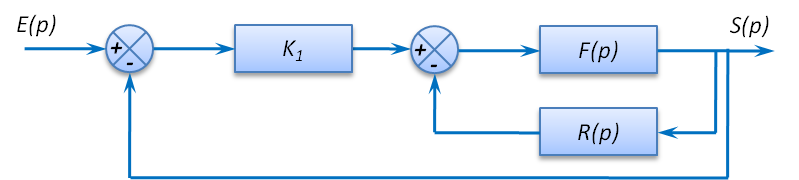
\includegraphics[width=.6\textwidth]{png/fig_03}
\end{center}

\subparagraph{}
\textit{Calculer la fonction de transfert $H(p)$ du système.}
\ifthenelse{\boolean{prof}}{
\begin{corrige}
\begin{center}
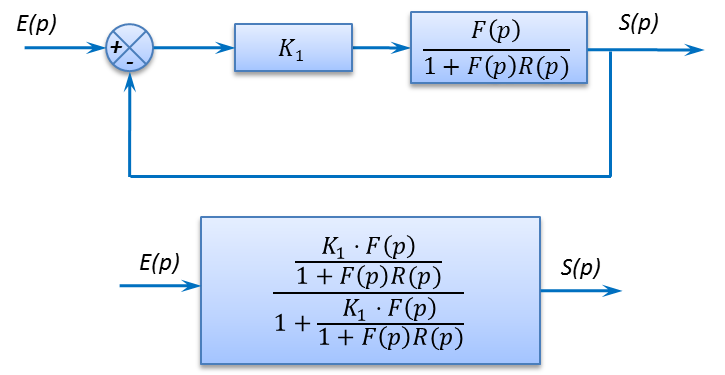
\includegraphics[width=.6\textwidth]{png/fig_03_Corr}
\end{center}

$$
\dfrac{S(p)}{E(p)} = \dfrac{K_1 F(p)}{1+F(p)R(p)+K_1 F(p)}
$$

\end{corrige}
}{}

On donne pour valeur aux différents blocs $F(p)=\dfrac{8}{p\left(p+4 \right)\left( p+5\right)}$, $R(p)=p$ et $K_1 = 5$.

\subparagraph{}
\textit{Calculer $H(p)$.}
\ifthenelse{\boolean{prof}}{
\begin{corrige}
On remplace les fonctions de transfert par leurs valeurs : 
$$
\dfrac{S(p)}{E(p)} = \dfrac{K_1 \dfrac{8}{p\left(p+4 \right)\left( p+5\right)}}{1+\dfrac{8p}{p\left(p+4 \right)\left( p+5\right)}+K_1 \dfrac{8}{p\left(p+4 \right)\left( p+5\right)}}
= \dfrac{8 K_1}{p\left(p+4 \right)\left( p+5\right)+8p+8 K_1 }
$$
\end{corrige}
}{}


\subsection*{Exercice 3}
\setcounter{subparagraph}{0}

Déterminer la sortie $S(p)$ et éventuellement la fonction de transfert correspondant aux schémas suivants : 

\begin{center}
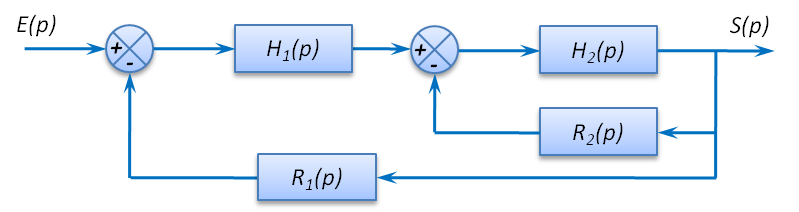
\includegraphics[width=.6\textwidth]{png/fig_04}
\end{center}

\ifthenelse{\boolean{prof}}{
\begin{corrige}
\begin{center}
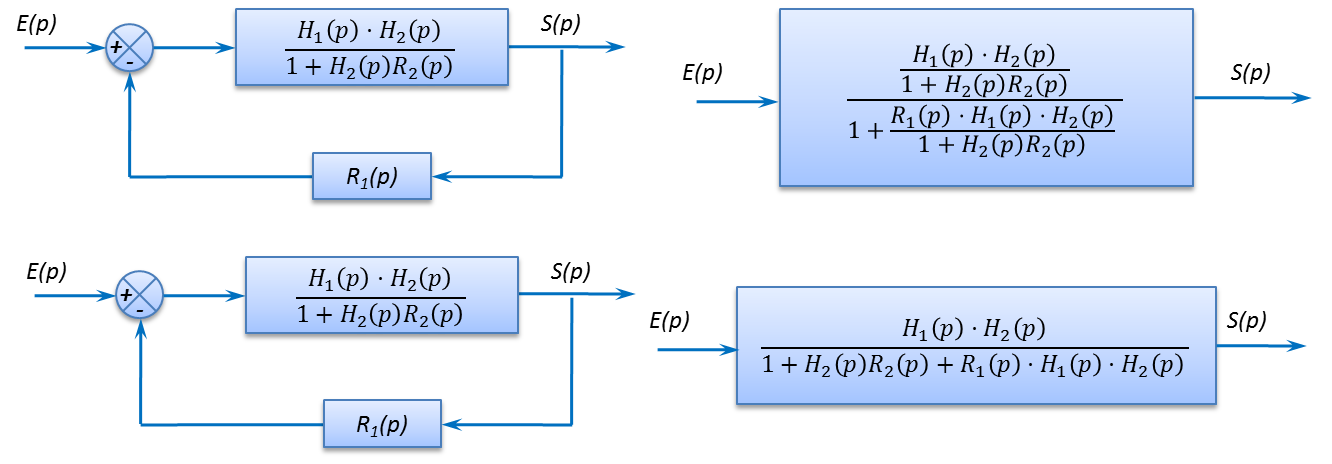
\includegraphics[width=.9\textwidth]{png/fig_04_Corr}
\end{center}
\end{corrige}
}{}

\begin{center}
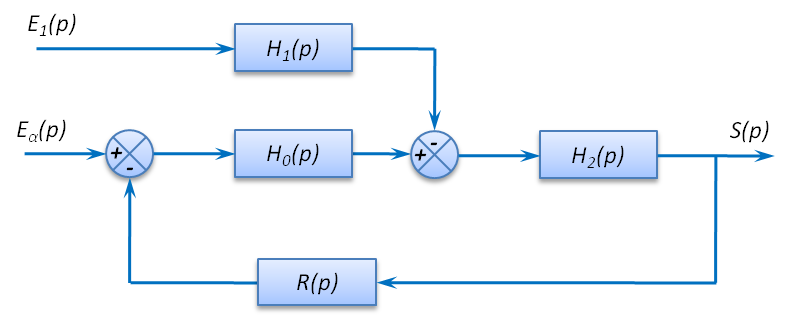
\includegraphics[width=.6\textwidth]{png/fig_05}
\end{center}


\ifthenelse{\boolean{prof}}{
\begin{corrige}
On note $G_1(p)=\dfrac{S(p)}{E_\alpha (p)}$ lorsque $E_1(p)=0$ : 
$$
G_1(p)=\dfrac{H_0(p)\cdot H_2(p)}{1+H_0(p)\cdot H_2(p)\cdot R(p)}
$$

On note $G_2(p)=\dfrac{S(p)}{E_1(p)}$ lorsque $E_{\alpha}(p)=0$ :
$$
G_2(p)=-H_1(p)\cdot \dfrac{H_2(p)}{1+H_0(p)\cdot H_2(p)\cdot R(p)}
$$

Au final, 
$$
S(p)=G_1(p)E_{\alpha}(p) + G_2(p) E_1(p)
$$
\end{corrige}
}{}


\begin{center}
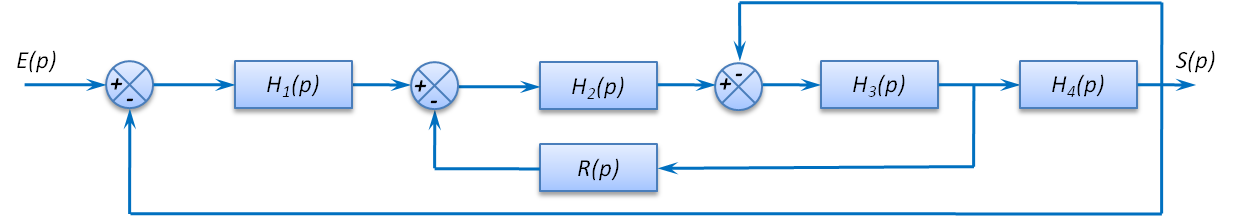
\includegraphics[width=.9\textwidth]{png/fig_06}
\end{center}

\ifthenelse{\boolean{prof}}{
\begin{corrige}
\begin{center}
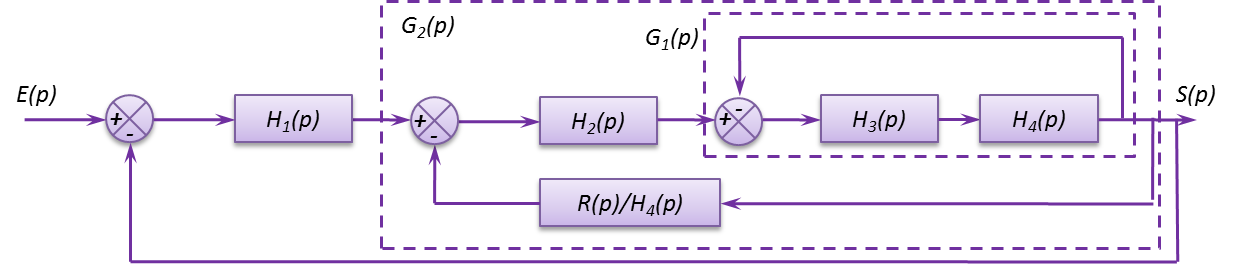
\includegraphics[width=.9\textwidth]{png/fig_06_Corr}
\end{center}
On a :
$$
G_1(p)=\dfrac{H_3(p)\cdot H_4(p)}{1+H_3(p)\cdot H_4(p)}
$$

$$
G_2(p) = 
\dfrac{H_2(p)\cdot G_1(p)}{1+H_2(p)\cdot G_1(p)\cdot\dfrac{R(p)}{H_4(p)}}
= 
\dfrac{H_2(p)\cdot \dfrac{H_3(p)\cdot H_4(p)}{1+H_3(p)\cdot H_4(p)}}{1+H_2(p)\cdot \dfrac{H_3(p)\cdot H_4(p)}{1+H_3(p)\cdot H_4(p)}\cdot\dfrac{R(p)}{H_4(p)}}
= 
\dfrac{H_2(p)\cdot H_3(p)\cdot H_4(p)}{1+H_3(p)\cdot H_4(p)+H_2(p)\cdot H_3(p)\cdot R(p)}
$$

Au final, 
$$
H(p)=\dfrac{H_1(p)\cdot G_2(p)}{1+H_1(p)\cdot G_2(p)}
=
\dfrac{H_1(p)\cdot \dfrac{H_2(p)\cdot H_3(p)\cdot H_4(p)}{1+H_3(p)\cdot H_4(p)+H_2(p)\cdot H_3(p)\cdot R(p)}}{1+H_1(p)\cdot \dfrac{H_2(p)\cdot H_3(p)\cdot H_4(p)}{1+H_3(p)\cdot H_4(p)+H_2(p)\cdot H_3(p)\cdot R(p)}}
$$
$$
H(p)=
\dfrac{H_1(p)\cdot H_2(p)\cdot H_3(p)\cdot H_4(p)}{1+H_3(p)\cdot H_4(p)+H_2(p)\cdot H_3(p)\cdot R(p)+H_1(p)\cdot H_2(p)\cdot H_3(p)\cdot H_4(p)}
$$
\end{corrige}
}{}


\end{document}
